
\lettrine[lines=3]{T}{}here are two major parts necessary to procedurally generate plant-life using an L-system. These are the rewriter and the interpreter. The purpose of the L-system rewriter is to take an L-system file as input, and generate the resulting string that fits the L-system grammar. It does this by syntactically and semantically analysing the L-system input, and generating the structures and information necessary to carry out the rewriting process. The rewriting process uses the structures and information, such as the string of modules and the production rules, to step through each string and rewrite the symbols. This chapter focuses on each part of the string rewriters' implementation and will introduce a technique of processing the L-systems' input, similar to how computer languages are compiled. This chapter will also formally define the L-system grammar in Backus-Naur Form, and provide the pseudocode for the L-system rewriter. 

For a simple D0L-system, like the one seen in section \ref{DOL-system example}. Each symbol within the alphabet is made up of a single character, the productions rules then match against those characters. As the D0L-system is deterministic, there is no randomness when determining the matching rule. The simplicity of the L-system makes it quite easy to create a rewriting system for the D0L-system. All the rewriter must do is store the starting string and production rule predecessors and successors. It then iterates over a string of symbols and replace them with the successor. The implementation of a more sophisticated L-system, like the parametric 0L-system, is much more complex. A parametric L-system can have multiple modules that make up a string, where each module may have multiple parameters, and each parameter could be a mathematical expression. The added complexity makes developing a rewriting system considerably more difficult. The rewriter must better understand what the syntax of the L-system is specifying, based on the context of each symbol within the L-system.

Due to the complexity of the L-system grammar, it is difficult for a computer to tell the syntactic and semantic properties of each part of the L-system input, which makes it difficult to carry out the rewriting process. Using a system similar to a \say{compiler}, an L-system "program" can be broken down into a three-stage process, as seen in figure \ref{3D rotations} below. The first stage is \textit{lexical analysis}, then a process called \textit{parsing} and finally the string rewriting stage. The lexical analyser is responsible for splitting the input into syntactic words, and then assigning each word into its syntactic category. Any word within the L-system that does match a syntactic category will result in a lexical error. If there are no lexical errors the words and their syntactic categories are sent to the parser. The parser matches the syntactical categories of each sentence in the language against a grammatical model. If any of the sentences within the language do not match the grammatical model, an appropriate error message can be displayed, similar to that of the lexical error. The error states where the syntax error occurred and what was grammatically incorrect. The parser also creates a syntax tree along with any data structures necessary for the rewriting process. These structures can then be used to carry out string rewriting or provide information to the interpreter.

\begin{figure}[htbp]
	{\centering
		\setlength{\fboxrule}{1pt}
		\vspace{7px}
		\fbox{
			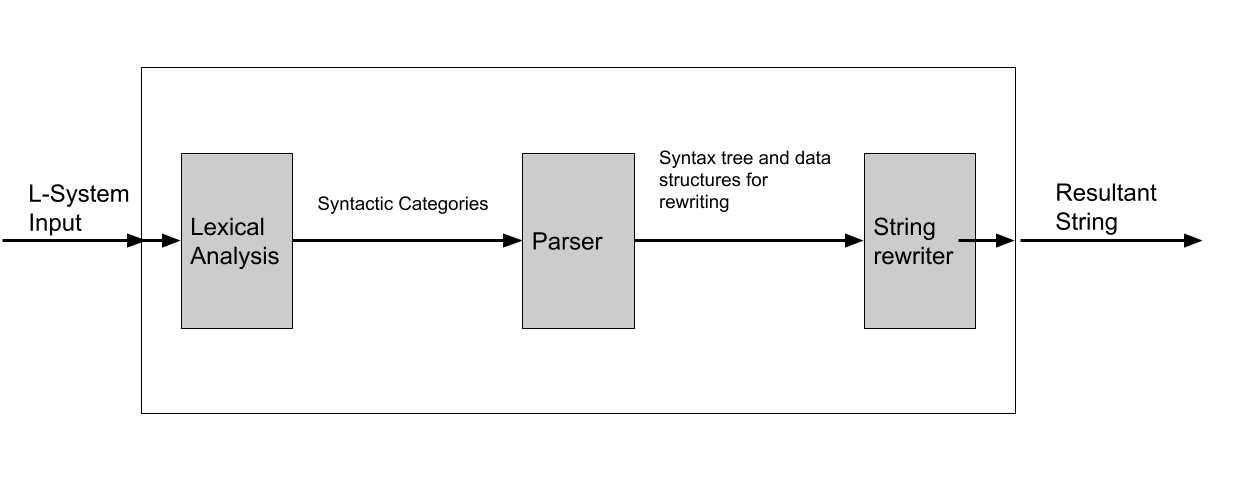
\includegraphics[scale=0.32]{Diagrams/StringRewriter.png}
		}
		\caption{Diagram of the Parts of The Rewiting System.} \label{3D rotations}
	}
\end{figure}
\FloatBarrier

\section{Environment and Tools}

The implementation of the string rewriter, and the string interpreter, is written in the C and C++ programming languages \cite{stroustrup2000c++}. The C and C++ languages are two of the most common programming languages that have stood the test of time with the first version of C being released in 1974. These languages are frequently used within computer graphics, with some of the most popular game engines supporting either C or C++. Such as CryEngine, Unreal Engine, Source Engine, and more. The main reason for this is the high performance and low-level memory management that C and C++ provide, and the graphics programming frameworks such as OpenGL, Vulkan, and DirectX all having direct support for either C or C++. The C and C++ languages also have a large number of useful libraries that provide extra functionality.  

The implementation of the rewriter and the interpreter will use the modern Open Graphics Library (\gls{OpenGL}). The OpenGL framework is one of the industry standards for creating 3D graphics applications. It is a cross-platform API for interacting with the \acrshort{gpu} in a low-level way. The high-performance nature of OpenGL is essential, as displaying and simulating the L-system can be very graphically intensive \cite{sellers2013opengl} \cite{movania2017opengl}. OpenGL was initially intended to be an \acrshort{api} for the C and C++ programming languages. Therefore, both the programming language and graphics API have a strong emphasis on performance, which is necessary when procedurally generating and simulating plant-life.

For more specialised mathematics capabilities, the \acrfull{glm} library holds many mathematics classes and functions for conveniently dealing with structures such as vectors, matrices, and quaternions. This thesis will cover these mathematical concepts in chapter \label{maths chapter}; however, it is convenient to have these implemented and tested within a C++ library. Another important library is \acrfull{glfw} which is a multi-platform \acrshort{api} for creating an managing user interface windows, events, and user-input \cite{glfwDocumentation}. To keep track of changes and manage versions. Git is a free and open-source version control software. It can keep track of changes that have been made to the files within a project folder as well as keep previous versions of the project throughout the development process. In conjunction with Git,  Github is an online web application that stores git repositories. Git acts as a backup as well as containing all previous versions of the project \cite{torvalds}.

\section{The L-system as an Interpreted Grammar}

Traditionally an interpreter in computing is a program that takes program code as input. It is then analyzed and interpreted as it is encountered in the execution process. All of the previously encountered information is kept for later interpretations. The information about the program can be extracted by inspecting the program, such as the set of declared variables in a block or a function \cite{wilhelm2010compiler}. In essence, the L-system rewriter contains a type of interpreter. This should not be confused with the interpreter that processes the resultant string using turtle graphics. Due to this confusion of terms, the system containing the lexical analyser, L-system parser, and the string rewriter will be referred to as the L-system rewriter, instead of the interpreter in the computational sense. 

A similarity can be drawn between traditionally interpreted languages and the L-system rewriter. The L-system rewriter defines a set of constant variables, a starting point, and then some production rules. This information can then be used to rewrite the starting string several times. Later on, it may be decided that, instead of five generations of rewriting, the rewriter should instead generate ten. Some information about the L-system is still valid, the production rules, axiom, and constants have not changed, and therefore this information can be used to interpret to the tenth generation. This concept can be used to go from the current state of the L-system rewriter and rewrite another five times. Instead of throwing all the information away and starting from scratch. Furthermore, if we would like to retrieve the resultant string, this can be requested from the L-system rewriter. 

The lexical analyser and parser are a necessary part to carry out rewriting. Without the lexical analyser or parser, it would not be straightforward to find the syntactic roles of each part of the L-system. Take the example of the module: F(2*3, x * (2 + y)). Here there is a single module with two parameters, one parameter has the expression (2 * 3), and the other has the expression (x * (2+y)). These complex structures within a grammar require knowledge about the grammatical model it represents. The lexical analyser firstly makes sure that all the syntax within the L-system is correct and assigns each word or symbol to a syntactic category, the parser then splits the L-system into its components and is describes each parts syntactic roll. The lexical analyser provides the understanding that x and y are variables within a module and do not represent something else. It also provides knowledge about how to find the values of x and y. 

The difficulty of creating an L-system with more complexity in the grammar is that it becomes more challenging to write a valid L-system to represent a particular structure. For example, imagine trying to write a C program where the compiler does specify why the program is incorrect. The advantage of using a rewriter similar to a compiler is that it makes it simpler to debug any syntactic errors, as well as make the string rewriting much faster. This means that writing an L-system becomes similar to rewriting a recursive program, where any syntactic mistakes will result in a meaningful error describing what was incorrect.

\section{The Syntax of a Parametric L-system}

This section will specify the valid syntax for the parametric L-system rewriter. The syntax is similar to the definition of the parametric L-system definition given by Prusinkiewicz and Lindenmayer in section \ref{definition of a parametric 0L-system section}. There are some additions and modifications to the syntax definition provided by Prusinkiewicz and Lindenmayer to construct an L-system that includes branching, constant variable definitions, object specifications, parametric L-system concepts, randomness, and stochastic L-systems \cite{prusinkiewicz2012algorithmic}. 

This L-system has five major parts. Each part is categorised as a statement. Valid statements are the \textit{defines} , the \textit{includes}, a single generation statement, a single axiom statement, and one or more production rules \cite{prusinkiewicz2013lindenmayer}. All of these statements collectively form an L-system. Each statement starts with a `\#' character and ends with a `;' symbol. These are used to indicate the start and end of a statement, even if multiple statements are written on the same line. 

The order that statements should be listed is as follows: 

\begin{equation} \label{statement order example}
\begin{aligned}
	&\text{\#generations statement;}\\
	&\text{\#define statements;}\\
	&\text{\hspace{10mm}...}\\
	&\text{\#include statements;}\\
	&\text{\hspace{10mm}...}\\
	&\text{\#axiom statement;}\\
	&\text{\#production statements;}\\
	&\text{\hspace{10mm}...}\\
\end{aligned}
\end{equation}

The order for the statements does not always matter; for instance, the generation statement can be defined anywhere within the L-system. However, some parts are required to be in a particular order, such as the define and include statements, which must appear above the axiom and production rule statements as they define values used within the axiom and production rules. It is best practice to specify the L-system in the above order as to avoid any conflictions or errors.

All numbers within the L-system are represented as floating-point numbers. Using a single data-type keeps all numbers consistent. Other data types could be added in the future; however, there are added complexities in doing so, such as the conversion from one type to another, or having to specify which data type a variable represents. The floating-point data type provides all the necessary functionality needed for the L-system; therefore, it seems unnecessary to add more data types. 

\section{The L-system Lexical Analyser} \label{Flex}

In computer science, specifically the study of programming language compilers, the program responsible for carrying out lexical analysis is the lexer. Depending on the literature the lexer can also be known as the tokenizer or scanner. D. Cooper and L. Torczon write that ``The scanner, or lexical analyser, reads a stream of characters and produces a stream of words. It aggregates characters to form words and applies a set of rules to determine whether each word is legal in the source language. If the word is valid, the scanner assigns it a syntactic category or part of speech'' \cite{cooper2011engineering}. This is no different for the parametric 0L-system rewriter. For the rewriter to have enough information to carry out rewriting, it must first understand what each word or token within the L-system means, this requires assigning a syntactic category to each token, and whether or not the token is valid or not within the L-system grammar.  

The scanner itself is quite complex, its main goal is to match the characters or strings within the language, to either a word or a regular expression defined in the grammar. When the match is made the token is given a syntactic category. The mechanism by which it achieves this is known as \textit{finite automata} \cite{wilhelm2013compiler}. It is possible to write custom \gls{Lexer}, however, it can be quite complicated and time-consuming to design and implement, and once a custom \gls{Lexer} has been created it is also difficult to change functionality at a later stage. There is a well known program known as the \acrlong{flex} (\acrshort{flex}). \acrshort{flex} takes in a file which contains the lexical rules of the language, this being the strings as well as the regular expression as well as its associated syntactic category. When \acrshort{flex} is executed it will create a \gls{Lexer} in the form of a C program. To create a lexer with \acrshort{flex}, the lexical rules must be defined. Below are the characters, strings and regular expressions and their associated syntactic categories, as well as a description as to its use in the parametric 0L-system. 

\begin{table}[h!] \center
\begin{tabular}{  c | l | l }

	Syntactic Word	& Syntactic Category & Description\\  
\hline
\hline
	, 				& T\_COMMA 				& Separation between module parameters \\

	: 				& T\_COLON 				& Separation between production rule parts \\

	; 				& T\_SEMI\_COLON 		& End of a statement\\

	\#				& T\_HASH 				& Beginning of a statement\\

	( 				& T\_PARENL 			& Start of a modules parameters \\
					&						& or specifies presidence in an expression \\

	) 				& T\_PARENR 			& End of a modules parameters \\
					&						& or specifies presidence in an expression \\
 
	\{ 				& T\_BRACKETL 			& Start of a random range\\

	\} 				& T\_BRACKETR 			& End of a random range\\

	$\sim$ 			& T\_TILDE 				& Stochastic operator\\

	== 				& T\_EQUAL\_TO 			& Relational operator stating equal to\\

	!= 				& T\_NOT\_EQUAL\_TO 	& Relational operator for not equal to\\
	
	$<$ 			& T\_LESS\_THAN 		& Relational operator for less than\\

	$>$ 			& T\_GREATER\_THAN 		& Relational operator for greater than\\

	$<$ = 			& T\_LESS\_EQUAL 		& Relational operator for greater or equal\\

	$>$ = 			& T\_GREATER\_EQUAL 	& Relational operator for greater or equal\\

	[ 				& T\_SQUARE\_BRACEL 	& Module name (branching save state) \\

	] 				& T\_SQUARE\_BRACER 	& Module name (branching load state) \\

	+ 				& T\_PLUS 				& Arithmetic operator for addition, or\\
					&						& Module name (Yaw right) \\

	- 				& T\_MINUS 				& Arithmetic operator for subtraction, or\\
					&						& Module name (Yaw left)\\

	/ 				& T\_FORWARD\_SLASH 	& Arithmetic operator for division, or\\
					&						& Module name (Pitch up)\\

	$\backslash$ 		& T\_BACK\_SLASH 		& Module name (Pitch down)\\

	* 				& T\_STAR 				& Arithmetic operator for multiplication, or\\
					&						& Condition in a production rule which is true\\

	$\land$		& T\_HAT 				& Arithmetic operator for and exponent, or\\
					&						& Module name (Roll right)\\

	$\&$ 			& T\_AMPERSAND 			& Module name (Roll left)\\

	! 				& T\_EXCLAMATION 		& Module name (Set size of branch)\\

	\$ 				& T\_DOLLAR 			& Module name \\

	= 				& T\_ASSIGN 			& Assignment operator used to set generations\\

	\#n 			& T\_GENERATIONS 		& Declaration of the number of generations\\

	\#w 			& T\_AXIOM 				& Declaration of the axiom\\

	\#define 			& T\_DEFINE 		& Declaration of the define\\

	\#object 			& T\_OBJECT			& Declaration of the object\\

	[0-9]+.[0-9]+$|$[0-9]+ 					& T\_FLOAT 				& Regular expression for a floating point number\\

	[a-zA-Z\_][a-zA-Z0-9\_]*  				& T\_VAR\_NAME 			& Regular expression for a module or variable name\\
\end{tabular}
\caption{Table of Valid Lexer Words}
\label{lexer words}
\end{table}
\FloatBarrier

\noindent
From the table above there are a number syntactic categories that contain more than one meaning to the grammar, for instance, the open and close parenthesis have two meanings, it is either to specify the beginning and end of a module's parameters or it specifies precedence within an expression.  It is not up to the scanner to determine what each parenthesis means, or that it has a meaning at all, the lexer only recognises that it falls into the syntactic categories, T\_PARENL and T\_PARENR. Deriving the meaning of a given token or syntactic category is left up to the parser which is more aware of the context of each syntactic word. Similarly, the symbols [,],+,-,/,$\backslash$, $\land$, $\&$, ! and \$ are valid module names; Moreover, it is possible for a T\_VAR\_NAME to also be a module name, these symbols need to be specifically defined as their syntactic category, as they not only represent a module name but can also represent a different meaning depending on their context. For instance, the +, -, / are valid module names, but they also are mathematical symbols used within an arithmetic expression. The scanner must separate these symbols and keep them in their syntactic category for the parser to be able to understand the same symbol in multiple contexts. 

It is also important to note that there are two special types of tokens, these being the T\_FLOAT and T\_VAR\_NAME which not only are part of a syntactic category but also contain a value, for instance, T\_FLOAT has a floating-point value and T\_VAR\_NAME has a string value. These values must be kept and provided to the parser.

\section{The L-system Parser} \label{parser}

The parsers' job is to find out if the input stream of words from the \gls{Lexer} makes up a valid sentence in the language. The \gls{Parser} fits the syntactical category to the grammatical model of the language. The \gls{Parser} can fit the syntactical categories from the lexer to the grammatical model of the language, if the syntactical categories match the grammatical model then the syntax is seen to be correct. If all of the syntax is correct the \gls{Parser} will generate a syntax tree and build the data structures for use later on in the compilation process \cite{cooper2011engineering}. For the L-system rewriter, the syntax tree and data structures are not used for compilation but rather for the string rewriting process. 

To describe a grammar, there needs to be a suitable notation to express its syntactic structure or grammatical model. According to Cooper the \acrshort{bnf} has traditionally been used by computer scientists to represent context-free grammars such as programming languages, its origins are from the late 1950s and early 1960s. The \acrlong{bnf} (\acrshort{bnf}) notation represents the context-free grammar by defining a set of non-terminal symbols that derives from a set of terminal or non-terminal symbols. Terminal symbols are elementary symbols of the language defined by the formal grammar, a terminal symbol will eventually appear in the resulting formal language. On the other hand, a non-terminal symbol exists only as a placeholder for patterns of terminal symbols but does not appear within the formal language itself. The syntactic convention for a \acrshort{bnf} is for non-terminal symbols to be surrounded by angled brackets. For instance $<$expression$>$ and terminal symbols, such as the symbol for addition \say{+} to be underlined, but nowadays it is not often underlined. The symbol $\epsilon$ represents an empty string, the ::= means \say{derives} and the $\mid$ means \say{also derives} but is often articulated as an \say{or} \cite{cooper2011engineering}. To derive a sentence of text within a language the very first derivation must be a non-terminal symbol called the goal symbol. The goal symbol is a set of all valid derived strings, this means that the goal symbol is not a word within the language, but rather a syntactic variable in the form of a non-terminal symbol. The \acrshort{bnf} notation below can be used to represent a simple grammar for arithmetic expressions, where the terminal \say{number} is any valid integer and the goal symbol is $<$expression$>$. Below is the \acrshort{bnf} notation for the syntax of an arithmetic expression that can represent addition and subtraction.

\noindent
\begin{algorithm}
\begin{bnf*}
	\bnfprod{expression}
		{\bnfts{number}}\\
		\bnfmore{\bnfor \bnfts{(} \bnfpn{expression} \bnfts{)}}\\
		\bnfmore{\bnfor \bnfpn{expression} \bnfts{+} \bnfpn{expression}}\\
		\bnfmore{\bnfor \bnfpn{expression} \bnfts{-} \bnfpn{expression}}
\end{bnf*}
\end{algorithm}
\FloatBarrier

\noindent
The \acrshort{bnf} above states that the goal symbol non-terminal $<$expression$>$ derives from one of four states. Either a terminal number, or an expression contained within two parentheses, or two expressions either side of an addition terminal symbol, or two expressions either side of a subtraction terminal symbol. This type of notation is recursive in nature and allows the formal language to write expressions that exist within other expressions. For example the expression \say{5 + 10 - (20 + 2)} can be broken down into using the \acrshort{bnf} production rule forming a syntax tree as seen in figure \ref{syntax tree} below. In this case, the whole expression fits the grammatical model of the language, thus it be parsed, forming the syntax tree. An expression such as this one would create an expression tree data structure, which will be discussed in more detail in section \ref{expression tree}. Depending on the production rule for the non-terminal system being parsed an associated data structure may be created.

\begin{figure}[htbp]
	{\centering
		\vspace{7px}
		
		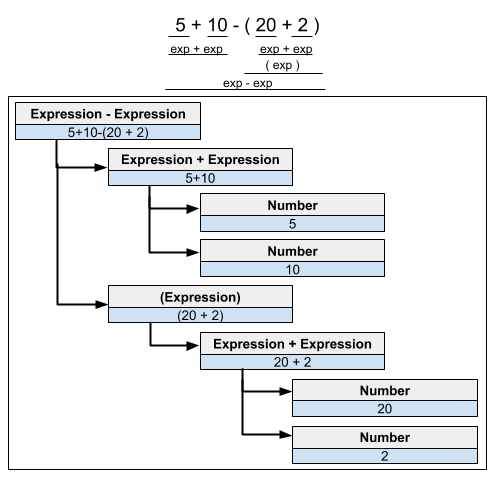
\includegraphics[scale=0.7]{Diagrams/syntaxTree.png}
		
		\caption{Diagram syntax tree for an expression.} \label{syntax tree}
	}
\end{figure}
\FloatBarrier

\noindent
Similar to the scanner, the parser program can be quite complex, as it needs to find the associated terminal and non-terminal symbols and comply with the grammatical model. Furthermore, if there is a change in the grammar or there is a need to add features at a later date, it is oftentimes difficult to change the parser to account for these changes. Many studies have been conducted on the optimal method of creating a parser, this is simply not the purpose of this thesis. Because of this, a program known as a parser generator will be used to create a parser program. It uses a specification of the grammar similar to that of the \acrshort{bnf} to generate a C program capable of parsing a given language. An implementation of a parser generator is called Bison.

\subsection{\acrlong{bnf} of the L-system Grammar} \label{L-system Grammar}
\begin{singlespace}
	\begin{bnf*}
	\bnfprod{lSystem}
		{\bnfes \bnfor \bnfpn{statements} \bnfsp \bnfts{EOF}}\\
	\bnfprod{statements}
		{\bnfes \bnfor \bnfpn{statement} \bnfpn{statements}}\\
	\bnfprod{statement}
		{\bnfts{EOL} \bnfor \bnfpn{generation} 
		\bnfor \bnfpn{definition} 
		\bnfor \bnfpn{object} 
		\bnfor \bnfpn{axiom} 
		\bnfor \bnfpn{production}}\\
	\bnfprod{generation}
		{\bnfts{\#define} \bnfsp \bnfts{=} \bnfsp \bnfpn{float} \bnfts{;}}\\
	\bnfprod{float}
		{\bnfts{[0-9]+.[0-9]+$|$[0-9]+}}\\
	\bnfprod{variable}
		{\bnfts{[a-zA-Z\_][a-zA-Z0-9\_]*}}\\
	\bnfprod{number}
		{\bnfpn{float} \bnfor \bnfts{-} \bnfsp \bnfpn{float}}\\
	\bnfprod{range}
		{\bnfts{\{} \bnfpn{number} \bnfts{,} \bnfpn{number} \bnfts{\}}}\\
	\bnfprod{definition}
		{\bnfts{\#define} \bnfsp \bnfpn{variable} \bnfsp \bnfpn{number} \bnfts{;}}\\
	\bnfprod{object}
		{\bnfts{\#object} \bnfsp \bnfpn{variable} \bnfsp \bnfpn{variable} \bnfts{;}}\\ 
	\bnfprod{module}
		{\bnfpn{variable} \bnfor \bnfts{+} 
		\bnfor \bnfts{-} 
		\bnfor \bnfts{/} 
		\bnfor \bnfts{$\backslash$} 
		\bnfor \bnfts{$\land$}
		\bnfor \bnfts{\&}
		\bnfor \bnfts{\$}
		\bnfor \bnfts{[}
		\bnfor \bnfts{]}
		\bnfor \bnfts{!}}\\
		\bnfmore{\bnfor \bnfts{+} \bnfts{(} \bnfpn{param} \bnfts{,} \bnfsp \bnfpn{paramList} \bnfts{)}}\\
		\bnfmore{\bnfor \bnfts{-} \bnfts{(} \bnfpn{param} \bnfts{,} \bnfsp \bnfpn{paramList} \bnfts{)}}\\
		\bnfmore{\bnfor \bnfts{/} \bnfts{(} \bnfpn{param} \bnfts{,} \bnfsp \bnfpn{paramList} \bnfts{)}}\\
		\bnfmore{\bnfor \bnfts{$\backslash$} \bnfts{(} \bnfpn{param} \bnfts{,} \bnfsp \bnfpn{paramList} \bnfts{)}}\\
		\bnfmore{\bnfor \bnfts{$\land$} \bnfts{(} \bnfpn{param} \bnfts{,} \bnfsp \bnfpn{paramList} \bnfts{)}}\\
		\bnfmore{\bnfor \bnfts{\&} \bnfts{(} \bnfpn{param} \bnfts{,} \bnfsp \bnfpn{paramList} \bnfts{)}}\\
		\bnfmore{\bnfor \bnfts{\$} \bnfts{(} \bnfpn{param} \bnfts{,} \bnfsp \bnfpn{paramList} \bnfts{)}}\\
		\bnfmore{\bnfor \bnfts{[} \bnfts{(} \bnfpn{param} \bnfts{,} \bnfsp \bnfpn{paramList} \bnfts{)}}\\
		\bnfmore{\bnfor \bnfts{]} \bnfts{(} \bnfpn{param} \bnfts{,} \bnfsp \bnfpn{paramList} \bnfts{)}}\\
		\bnfmore{\bnfor \bnfts{!} \bnfts{(} \bnfpn{param} \bnfts{,} \bnfsp \bnfpn{paramList} \bnfts{)}}\\
	\bnfprod{axiom}
		{\bnfts{\#w} \bnfsp \bnfts{:} \bnfsp \bnfpn{axiomStatementList} \bnfts{;}}\\
	\bnfprod{axiomStatementList}
		{\bnfes \bnfor \bnfpn{axiomStatement} \bnfpn{axiomStatementList}}\\
	\bnfprod{axiomStatement}
		{\bnfpn{module}}\\
	\bnfprod{paramList}
		{\bnfes \bnfor \bnfpn{param} \bnfpn{paramList}}\\
	\bnfprod{param}
		{\bnfpn{expression}}\\
	\bnfprod{expression}
		{\bnfpn{variable} \bnfor \bnfpn{number} \bnfor \bnfpn{range}}\\
		\bnfmore{\bnfor \bnfpn{expression} \bnfts{+} \bnfpn{expression}}\\
		\bnfmore{\bnfor \bnfpn{expression} \bnfts{-} \bnfpn{expression}}\\
		\bnfmore{\bnfor \bnfpn{expression} \bnfts{*} \bnfpn{expression}}\\
		\bnfmore{\bnfor \bnfpn{expression} \bnfts{/} \bnfpn{expression}}\\
		\bnfmore{\bnfor \bnfpn{expression} \bnfts{$\land$} \bnfpn{expression}}\\
		\bnfmore{\bnfor \bnfts{(} \bnfpn{expression} \bnfts{)}}\\
	\bnfprod{production}
		{\bnfts{\#} \bnfpn{variable} \bnfsp \bnfts{:} \bnfsp \bnfpn{predecessor} \bnfsp \bnfts{:} \bnfsp \bnfpn{condition} \bnfsp \bnfts{:} \bnfsp \bnfpn{successor} \bnfts{;}}\\
		\bnfprod{predecessor}
		{\bnfpn{predecessorStatementList}}\\
	\bnfprod{predecessorStatementList}
		{\bnfes \bnfor \bnfpn{predecessorStatement} \bnfpn{predecessorStatementList} }\\
	\bnfprod{predecessorStatement}
		{\bnfpn{module}}\\
	\bnfprod{condition}
		{\bnfts{*}}\\
		\bnfmore{\bnfor \bnfts{$\sim$} \bnfpn{float}}\\
		\bnfmore{\bnfor \bnfpn{leftExpression} \bnfpn{operator} \bnfpn{rightExpression}}\\
	\bnfprod{leftExpression}
		{\bnfpn{expression}}\\
	\bnfprod{rightExpression}
		{\bnfpn{expression}}\\
	\bnfprod{operator}
		{\bnfts{==} \bnfor \bnfts{!=} \bnfor \bnfts{$<=$} \bnfor \bnfts{$>=$} \bnfor \bnfts{$>$} \bnfor \bnfts{$<$}}\\
	\bnfprod{successor}
		{\bnfpn{successorStatementList}}\\
	\bnfprod{successorStatementList}
		{\bnfes \bnfor \bnfpn{successorStatement} \bnfpn{successorStatementList}}\\
	\bnfprod{successorStatement}
		{\bnfpn{module}}\\
	\end{bnf*}

\newpage

\end{singlespace} 

\noindent
As seen above in the \acrshort{bnf} notation for a L-system, the goal state is $<$lSystem$>$. The $<$lSystem$>$ can be made up of $<$statements$>$ beginning with the symbol \say{\#} and ending with the symbol \say{;}, or the \acrlong{eof} (\acrshort{eof}) character signifying the end of the L-system. Each non-terminal $<$statements$>$ is made up of a $<$statement$>$ followed by more $<$statements$>$, or an empty string ($\epsilon$). The $<$statement$>$ itself can either be an \acrlong{eol} (\acrshort{eol}) character or a $<$generation$>$, $<$definition$>$, $<$object$>$, $<$axiom$>$ or $<$production$>$ statement. The non-terminal symbols $<$float$>$ and $<$variable$>$ specify a regular expression. Each statement then has a number of terminal and non-terminal derivatives that allow the production of all valid L-systems that follow this grammar. 

In the previous chapter, the scanner defined the syntactic categories, these syntactic categories are all the valid terminal symbols within the L-system grammar. In essence, the parser takes these syntactic categories and finds if they fit the above \acrshort{bnf} and if so, it extracts the information from the L-system and generates the relevant data structures and syntax tree. 

\subsection{Dealing with Constant Values and Objects}

Defining constants and objects is similar syntactically, the keyword define or include is used, followed by a variable name followed by a value, the value for a constant is a floating-point number and the value for an \textit{include} is a name of an object within the predefined object library. An example of defining a constant and an object can be seen below: 

\begin{equation} \label{constant and object example}
\begin{aligned}
	&\text{\#define num 10;}\\
	&\text{\#define pi 3.1415;}\\
	&\\
	&\text{\#include F BRANCH;}\\
	&\text{\#include S SPHERE;}\\
\end{aligned}
\end{equation}

\noindent
The definition variables can be stored as a table, called a constants table, which keeps track of all of the constant variable names as well as their values defined by the L-system, as seen in the table below: 

\begin{table}[h!] \center
\begin{tabular}{ | c | l | }
\hline
	Variable Name 	& Value\\  
\hline
\hline
	num 				& 10.0\\
\hline
	pi					& 3.1415\\
\hline
\end{tabular}
\caption{Table of turtle instruction symbols and their meaning to the interpreter}
\label{constants table}
\end{table}
\FloatBarrier

\noindent
The object table structure is very similar to the constants table, the object table holds the module name, and name of the object in the predefined object library. The object table will not be used during rewriting but it will be necessary to provide information during the interpretation of the resulting string about which objects each module should render. 

\begin{table}[h!] \center
\begin{tabular}{ | c | l | }
\hline
	Module Name	& Object Name\\  
\hline
\hline
	F 				& BRANCH\\
\hline
	S				& SPHERE\\
\hline
\end{tabular}
\caption{Table of turtle instruction symbols and their meaning to the interpreter}
\label{constants table}
\end{table}
\FloatBarrier

\subsection{Implementing Modules and Strings} \label{modules and strings}

For the rewriter it is important to understand that there are three major parts of a module, there is a module name, which is a string of characters or a symbol, secondly, there is a list of parameters signified by open and close parenthesis, there can be zero or more parameters listed. If there are no parameters for a module you can specify it without parenthesis, however, there should then be a space between the module without parenthesis and the next module. Thirdly, each parameter can either be made up of a number, variable, random number range or a mathematical expression containing numbers, variables and parentheses signifying precedence. 

It is important to note that there are two types of modules. One being a module definition and the other a module call. Although these are two different types of modules, they can refer to the same thing. This is because the module definition stands as a template for a module within a production rule. These templates do not have to hold actual values but rather the variable names or random ranges which will be substituted during the rewriting process. Module calls, on the other hand, would appear either in the axiom or in the resultant string, the parameters of a module call will always hold actual numerical values. Below is an example outlining the difference between the module definition and module calls.

\begin{equation} \label{module definition and call example}
\begin{aligned}
	&\text{\#w : A(10, 20);}\\
	&\text{\#p1 : A(x, y) : * : A(x+y, y); }\\
\end{aligned}
\end{equation}

\noindent
In the example \ref{module definition and call example} above, module A(10, 20) within the axiom, is a module call, as it contains two numerical values of 10 and 20. In the production rule p1, the predecessor is the module A(x, y), this is a module definition, it states that module A's first parameter has a local variable x, and its second parameter has the local variable y. The calling modules values 10 and 20 will substitute x and y respectively, anywhere within the successor statement. The production rule p1's successor has a single module A(x+y, y), this is also a module definition, however, the variables will be substituted with the calling modules values such that it is A(10+20, 20). This can then be evaluated to A(30, 20). After the successor module has been substituted and evaluated, the successors' modules must have a numerical value. They then become module calls within the resultant string ready for the next round of rewriting.

A string in the context of a parametric L-system is a vector of modules, the modules are linked one after the other creating a type of string, but instead of characters or symbols, we have a string of modules.

\subsection{Implementing Arithmetic Expressions Trees} \label{expression tree}

As stated within the \acrshort{bnf} of the L-system grammar an expression is either a variable name, a number or a random range, it is also possible that an expression is part of another expression. Take the example: $5 \times 4 + n$, here there are three expressions 5, 4 and $n$ however, $5 \times 4$ is also an expression, as well as $4 + n$. An expression can also be described as any of the aforementioned expressions between a set of parentheses such as $(4+n)$. The result of the expression is calculated from left to right unless the parenthesis is used which prioritises the encapsulated expression to be calculated first. We can represent this expression as an expression tree in the diagram below:

\begin{figure}[htbp]
	{\centering
		\setlength{\fboxrule}{1pt}
		\vspace{7px}
		\fbox{
			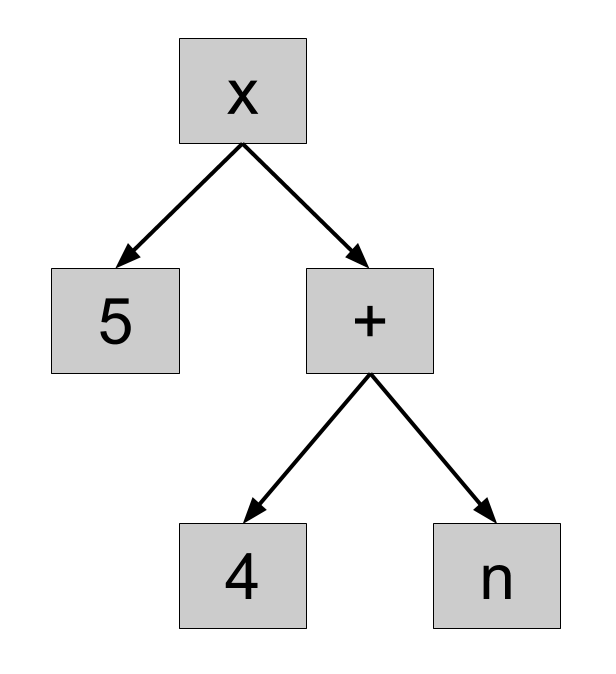
\includegraphics[scale=0.4]{Diagrams/ThesisContent.png}
		}
		\caption{Diagram of an expression tree.} \label{3D rotations}
	}
\end{figure}
\FloatBarrier

\noindent
The parser provides a syntax tree, which makes it easy to generate the above expression tree, this can have four types of nodes, a variable, number, random range or an operator. The end nodes of the expression tree must be either a number, variable or random range; moreover, a connecting node within the tree must be an operator. We can then traverse the generated tree, and replace the variables with their associated value, and for random ranges, we can generate the random value and assign it to the node. A second traversal during the rewriting process can then computes the result of the expression. 

\subsection{Implementing Random Ranges}

L-systems can be quite limited in the amount of variation that can be achieved from rewriting alone. In reality, the variation between the two plants depends on an enormous number of factors. Regardless of the cause, the factors ultimately change the variation mainly within the branching structure as well as a slight variation in the features of the branches themselves. These features include but are not limited to branching angles, branch width, branch length, and branch weight. To introduce variation in the branching structure the rules that are chosen need to be random now and then, which is discussed in section \ref{stochastic rules}. This section introduces a method of providing variation in the features of branch segments, will be called random ranges. 

A random range provides a method of declaring a variable that represents a number that should be randomly generated between two bounding numbers. The bounding numbers are the minimum and a maximum respectively. The main method used for generating a pseudo-random number using a uniform distribution within a range which can be seen below. 

\begin{singlespace}
\begin{algorithm}
\begin{algorithmic}[1]
\Procedure{Random Range}{min, max}
	\State n $\gets$ (rand() \% (max - min + 1)) + min
	\State \textbf{return} n
\EndProcedure
\end{algorithmic}
\end{algorithm}
\end{singlespace}

\noindent
Several other types of pseudo-random number generators can be used to generate numbers according to certain distributions; such as normal, binomial, Poisson among others. To generate plant-life a uniform distribution should be sufficient.

A random range can be declared in the define statement, axiom parameter or a production rule successor parameter. If it is declared within a define statement, it will generate a random number when that constant variable is added to the constants table. A random range declared within the axiom will generate a random number before the string rewriting process begins, this ensures that the number. And finally, if a random range is defined within the successor of a production rule, the number should be generated during the rewriting process when the current module within the string is successfully matched to the predecessor at the same time as the expressions within the successors are being evaluated. The values are generated during the rewriting process rather than prior is so that each time a module is matched to the rule, the successor will generate a different value.

\subsection{Implementing Stochastic Rules} \label{stochastic rules}

Each rule belonging to a stochastic group of rules provides a probability value of how likely it is that the particular rule is selected during the rewriting process. For production rules to be part of the same stochastic group they are required to meet four criteria: 

\begin{itemize}
\item The stochastic operator $\sim$ must be used with a probability between 0.0 and 1.0.
\item The predecessor module name must match the other predecessor module names within that stochastic group.
\item The number of parameters within the predecessor must match the number of parameters of other production rules within that stochastic group.
\item The total probability of all of the production rules within the stochastic group must not exceed 1.0 or be less than 0.0.
\end{itemize}

Each time a rule is added to a stochastic group an entry a stochastic rule table is created to keep track of which rules are associated with which stochastic group as well as the probability of each rule. Using the stochastic rules below, we can generate a stochastic rule table as seen in table \ref{stochastic table}. 

\begin{equation} \label{stochastic implementation example}
\begin{aligned}
	&p_1~ :  F(x)~ :~ \sim 0.33 ~ :~ F(x)[+(r)F(x)]F(x)[-(r)F(x)]F(x)\\
	&p_2~ :  F(x)~ :~ \sim 0.33 ~ :~ F(x)[+(r)F(x)]F(x)\\
	&p_3~ :  F(x)~ :~ \sim 0.34 ~ :~ F(x)[-(r)F(x)]F(x)\\
\end{aligned}
\end{equation}

\begin{table}[h!] \center
\begin{tabular}{ | c | c | c | }
\hline
	Stochastic Group & Rule Name & Probability\\  
\hline
\hline
\multirow{3}{*}{F1} & p1 & 0.33 \\
& p2 & 0.33 \\
& p3 & 0.34 \\
\hline
\end{tabular}
\caption{Table of the stochastic rules probabilities within a stochastic group.}
\label{stochastic table}
\end{table}
\FloatBarrier

The stochastic name can be generated by using the module name of the predecessor of the production rule as well as the number of parameters within the predecessor module. In the example above we can use the predecessor name F which has a single parameter, making the stochastic name F1. This serves as a unique identifier for the stochastic group. Once all of the production rules have been processed and added to the stochastic rule table, each groups' probabilities should be added together and the total should equal 1.0, certain tolerances should put in place to account for floating-point error. 

During the rewriting process, the module that is to be rewritten will be matched to a particular stochastic group. A uniformly distributed random number is then generated between 0.0 and 1.0. A range for each rule will then be generated, for instance, p1 will be between 0.0 and 0.33, p2 will be between 0.33 and 0.66 and finally, p3 will be between 0.66 and 1.0. The production rule with the range that the random number falls between is then selected and used for rewriting. 

\section{The String Rewriter}

Once the L-system has been processed by both the lexical analyser and the parser, the data structures and information is set up for the string rewriter. The string rewriter is the final stage which uses this data by starting with a current string of modules which is originally set to the axiom string. The string rewriter will then iterate over each module within the current string carrying matching it to the production rules and rewriting the module with the successor if the production rule matches. Once all of the modules have been rewritten, the current string is replaced by the result string for that iteration. This process is carried out for the number of generations specified within the L-system and will eventually provide the resultant string of modules.

When the string rewriter is run it should data for the number of generations, axiom string, production rules, constants table, and local variable table. Below is the pseudocode for the rewriting procedure as well as several useful functions for finding the matching production rule, replacing variables, evaluating expressions and adding variables to the local table. 

\begin{singlespace}
\newpage

\lstset{language=C}
\lstset{morekeywords=string}

\begin{lstlisting}[frame=single] 
struct node{
  enum Type {VARIABLE, OPERATOR, NUMBER, RANGE} type;
  union{
  	string *variable; 
  	string *operator; 
  	float number;
  	float range[3];
  };
  node *left; 
  node *right; 
};
\end{lstlisting}

\lstset{morekeywords=vector}
\lstset{morekeywords=node}

\begin{lstlisting}[frame=single] 
struct condition{
    enum Type {EQUAL_TO, NOT_EQUAL_TO, LESS_THAN, GREATER_THAN, 
    	LESS_EQUAL, GREATER_EQUAL, STOCHASTIC, NO_CONDITION} type;
    node * leftExp;
    node * rightExp;

    float stochasticValue;
};
\end{lstlisting}

\lstset{morekeywords=condition}

\begin{lstlisting}[frame=single] 
struct module{
  string name;
  int numParam; 
  enum Type {CALL, DEFINITION} type;
  string object; 
  vector<struct node*> params;
};
\end{lstlisting}

\lstset{morekeywords=module}

\begin{lstlisting}[frame=single] 
struct production{
    string name;
    module *predecessor;
    condition *condition;
    vector<module*> successor;
};
\end{lstlisting}

\newpage
\begin{algorithmic}[1]
\Procedure{rewriter}{N, A}
\Statex
\Ensure N $>$ 0																	\Comment{The number of generations to rewrite}
\Ensure A $\not=$ empty															\Comment{A non empty Axiom, a list of modules}
\Statex
\State n $\gets$ 0
\State current $\gets$ A														\Comment{Current string of modules}
\While{n $<$ N}																	\Comment{For each generation}
	\State next $\gets$ empty list
	\For{each mod in current}													\Comment{call is the calling module in current}
		\State P $\gets$ \Call{FindProductionMatch}{mod}						\Comment{P is the matching production rule}
		\If{P $\not=$ NULL}
			\State pred $\gets$ P.predecessor									\Comment{def is the defining module in predecessor}
			\For{each succ in P.successor}
				\State index $\gets$ 0
				\While{index $<$ number of predecessor parameters}
					\State \Call{AddLocalVar}{pred.param[index], mod.param[index]}
					\State index $\gets$ index + 1
				\EndWhile
				\State copy $\gets$ succ 										\Comment{Create a deep copy}
				\For{each parameter in copy}									\Comment{parameter is an expression tree}
					\State \Call{ReplaceVariables}{parameter}
					\State \Call{EvaluateExpression}{parameter}
				\EndFor
				\State next $\gets$ next + copy
			\EndFor
		\Else
			\State next $\gets$ next + mod
		\EndIf
	\EndFor
	\State n $\gets$ n + 1
	\State current $\gets$ next
\EndWhile
\State \textbf{return} current
\EndProcedure
\end{algorithmic}

\newpage
\begin{algorithmic}[1]
\Function{FindProductionMatch}{Module}
\For{each P in productionTable}												\Comment{P is a production}
	\State predecessor $\gets$ P.predecessor								\Comment{predecessor is a single module}
	\If{predecessor.name $\not=$ Module.name}
		\State \textbf{continue}
	\EndIf
	\If{predecessor.numParam $\not=$ Module.numParam}
		\State \textbf{continue}
	\EndIf
	\If{P has no condition}													
		\State \textbf{return} P.name										\Comment{match found}
	\ElsIf{P has a stochastic condition}
		\State rand $\gets$ random float between 0.0 and 1.0
		\State total $\gets$ 0.0
		\State S $\gets$ list of pairs 										\Comment{pair(production name, probability value)} 
		\For{each s in S}													\Comment{Loop through each tuple in the stochasic list}
			\If{first item}
				\If{rand $\geq$ 0.0 AND rand $<$ s.value}
					\State \textbf{return} s.name
				\EndIf
			\ElsIf{last item}
				\If{rand $\geq$ total AND rand $\leq$ 1.0}
					\State \textbf{return} s.name
				\EndIf
			\Else
				\If{rand $\geq$ total AND rand $<$ total + s.value}
					\State \textbf{return} s.name
				\EndIf
			\EndIf
			\State total $\gets$ total + s.value
		\EndFor	
	\Else																	\Comment{Regular condition}
		\State left $\gets$ P.condition.left								\Comment{Deep copy left expression tree}
		\State right $\gets$ P.condition.right								\Comment{Deep copy right expression tree}
		
		\State \Call{replaceVariables}{left}
		\State \Call{replaceVariables}{right}
		
		\State \Call{evaluateExpression}{left}
		\State \Call{evaluateExpression}{right}
		
		\If{left P.condition.op right}										\Comment{Apply operator ($==$, $\not=$, $<$, $>$, $\leq$, $\geq$)}
			\State \textbf{return} P.name
		\EndIf 																		 
	\EndIf							 
\EndFor
\EndFunction

\end{algorithmic}

\newpage
\begin{algorithmic}[1]

\Function{EvaluateExpression}{TreeNode}										\Comment{Recursively evaluate the expression tree}
	\State left $\gets$ 0.0									
	\State right $\gets$ 0.0
	
	\If{TreeNode.left $==$ NULL OR TreeNode.right $==$ NULL}
		\State \textbf{return} TreeNode.value
	\EndIf
	
	\State left $\gets$ \Call{ReplaceVariables}{TreeNode.left}
	\State right $\gets$ \Call{ReplaceVariables}{TreeNode.right}
	
	\If{TreeNode.type is an operator}
		\State \textbf{return} left TreeNode.operator right					\Comment{Apply arithmetic operator (+, -, *, /, $\land{}$)}
	\EndIf
\EndFunction
\\
\end{algorithmic}

\begin{algorithmic}[1]

\Function{ReplaceVariables}{TreeNode}										\Comment{Recursively replace expression tree variables}
	\If{TreeNode $==$ NULL}
		\State \textbf{return}
	\EndIf
	\If{TreeNode.type is a variable}
		\If{TreeNode.value is in constants table}
			\State TreeNode.value $\gets$ numeric value in constants table 
		\EndIf
		\If{TreeNode.value is in local table}
			\State TreeNode.value $\gets$ numeric value in local table
		\EndIf
	\EndIf
	\State \Call{ReplaceVariables}{TreeNode.left}
	\State \Call{ReplaceVariables}{TreeNode.right}
\EndFunction
\\
\end{algorithmic}

\begin{algorithmic}[1]

\Function{AddLocalVar}{TreeNodeCall, TreeNodeDef}
	\If{TreeNodeCall child nodes == NULL OR TreeNodeDef child nodes == NULL}
		\If{TreeNodeCall.type == Number AND TreeNodeDef.type == Variable}
			\State Add variable name and value to local table
		\ElsIf{TreeNodeCall.type == Range AND TreeNodeDef.type == Variable}
			\State Add variable and generated random range value to local table 
		\EndIf
	\EndIf
	
									
\EndFunction

\end{algorithmic}

\end{singlespace}

\newpage
\section{Summary}

The L-system rewriter is one of two major systems within the process or procedurally generating plant-life. The rewriter defined in this thesis acts as a type of compiler similar to that of a computer language. In a sense, the L-system itself becomes a language, that the L-system rewriter can understand and generate meaningful data structures with. The L-system rewriter follows the grammatical structure of the language very closely. Due to the lexer and the parser, it can give informative messages if there is a mistake either grammatically or syntactically. If all of these requirements are met, the rewriter can use this data to very quickly generate the resultant string of modules. The person writing that L-system, can know indefinitely that the result provided by the rewriting system is correct according to the grammar of the L-system.

The L-system languages can be used for many different applications and are not limited to that of procedural plant generation. The interpretation of the resultant string is really what creates the physical result such as the plant model. This means that this L-system rewriter need not change if the L-system is used for a different purpose, only the interpretation will need to change. This is the main reason behind using a compiler-like process to govern the string rewriting. It allows the L-system enough complexity to provide information to the interpreter but not too much that interpretation becomes reliant on the string rewriter.